\section{Appendici}

\begin{frame}
\frametitle{New era of Multimodal Unified Transformer}  
Google, Meta, Apple, OpenAI and many more company are working in a unified approach where images and text are processed together,
in order to provide a multimodel understanding of the world.
\begin{center}
    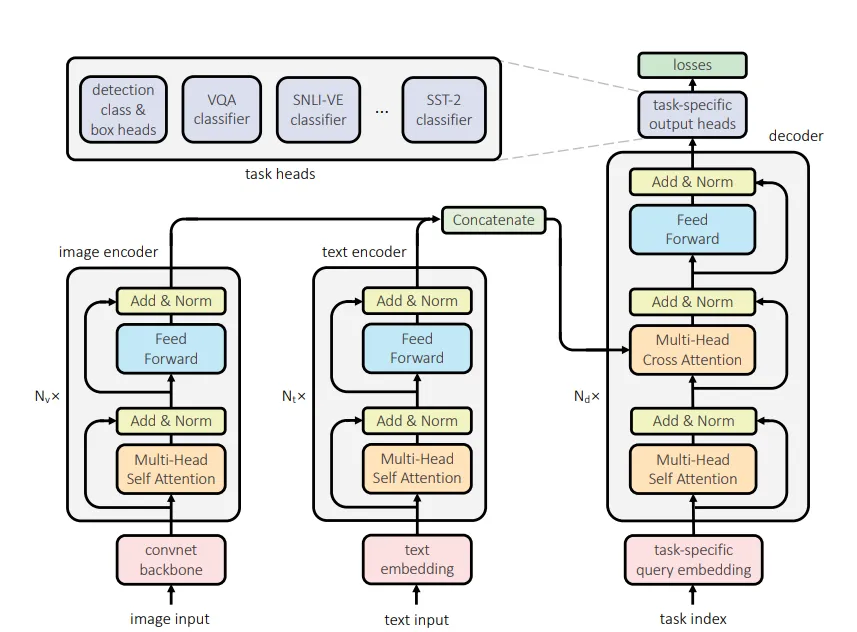
\includegraphics[width=0.6\textwidth]{img/4-section/Multimodel.png}
\end{center}

\end{frame}

\begin{frame}
    \frametitle{What type of Position Embedding?}
    
We can use a 1D or a 2D representation for Position Embedding

\begin{figure}
    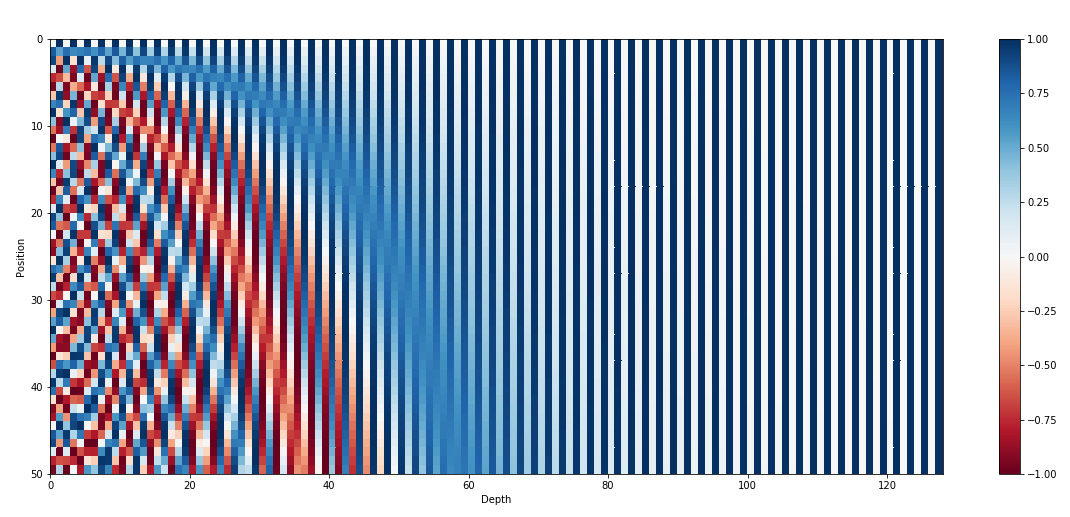
\includegraphics[width=0.8\textwidth]{img/2-section/positional_encoding.png} 
    \label{fig:Positional_encoding}
    \caption{Positional encoding matrix}
\end{figure}
\end{frame}


\begin{frame}
\frametitle{ConvNeXt more benchmark}
Push the limits of ConvNet potential, modernizing  standard ResNet towards a Transformer-like design.

\begin{center}
    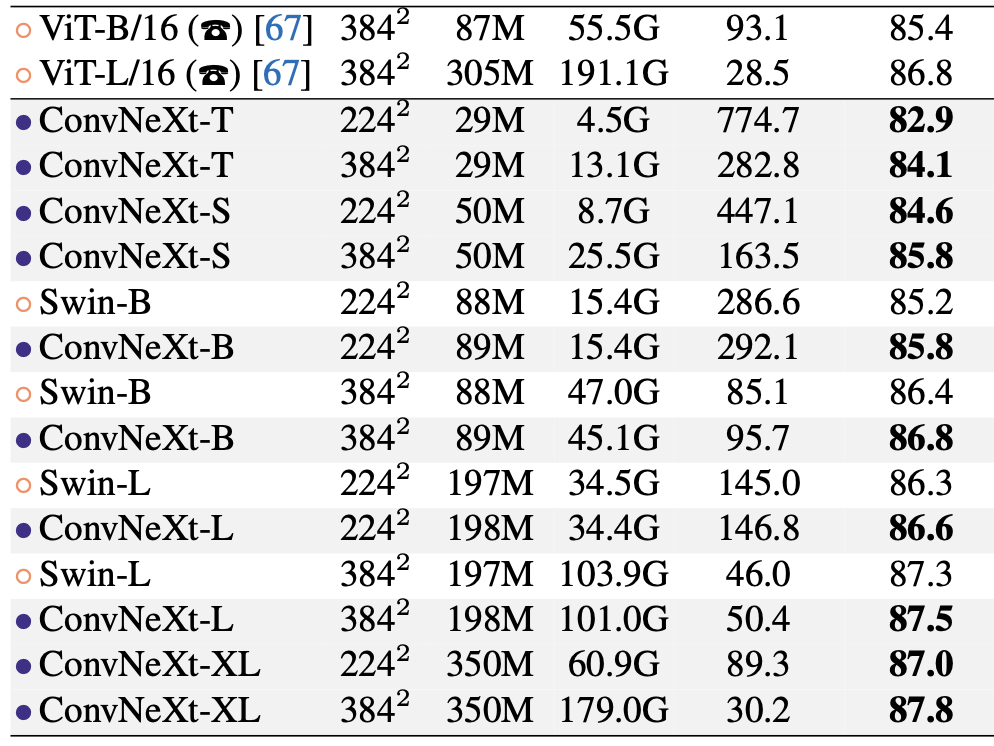
\includegraphics[width=0.5\textwidth]{img/4-section/ConvNext2.png}
\end{center}

Image site, \#param, flops, image/s, Top-1

\end{frame}


% \begin{frame}
% \frametitle{More Benchmark with ResNet}
% Benchmark between ResNet and ConvNeXt
% \begin{center}
%     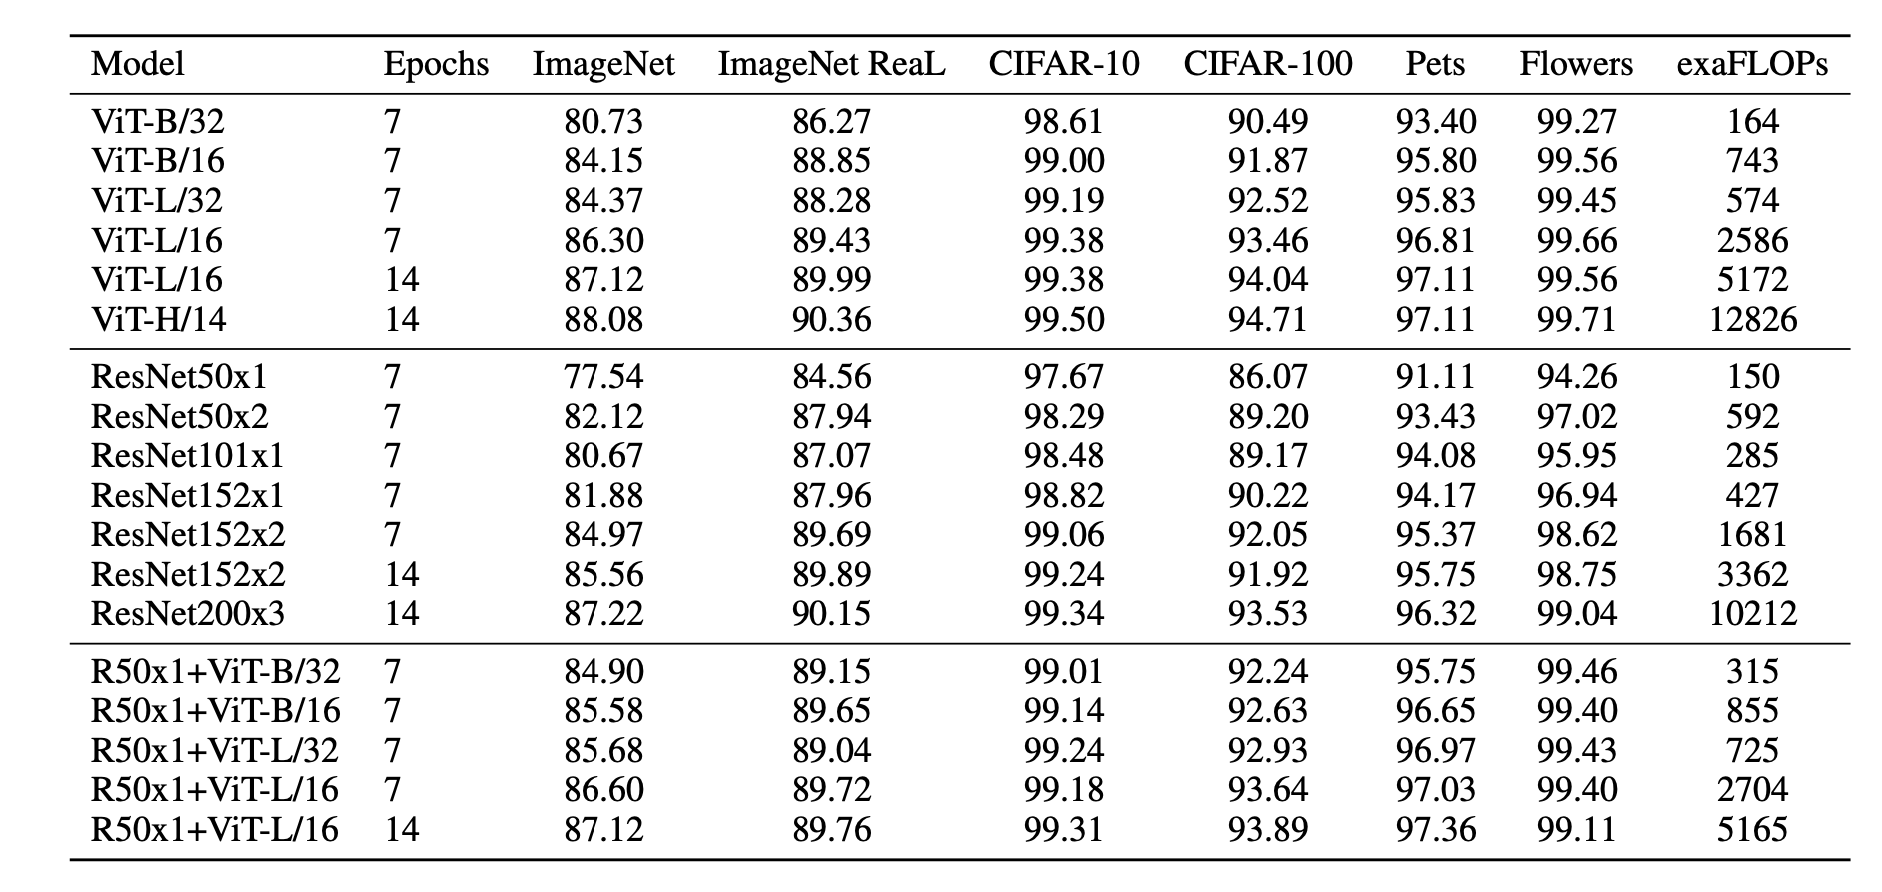
\includegraphics[width=1\textwidth]{img/4-section/More-benchmark.png}
% \end{center}

% \end{frame}

\begin{frame}
\frametitle{Different ViT models}
Benchmark between different ViT models
\begin{center}
    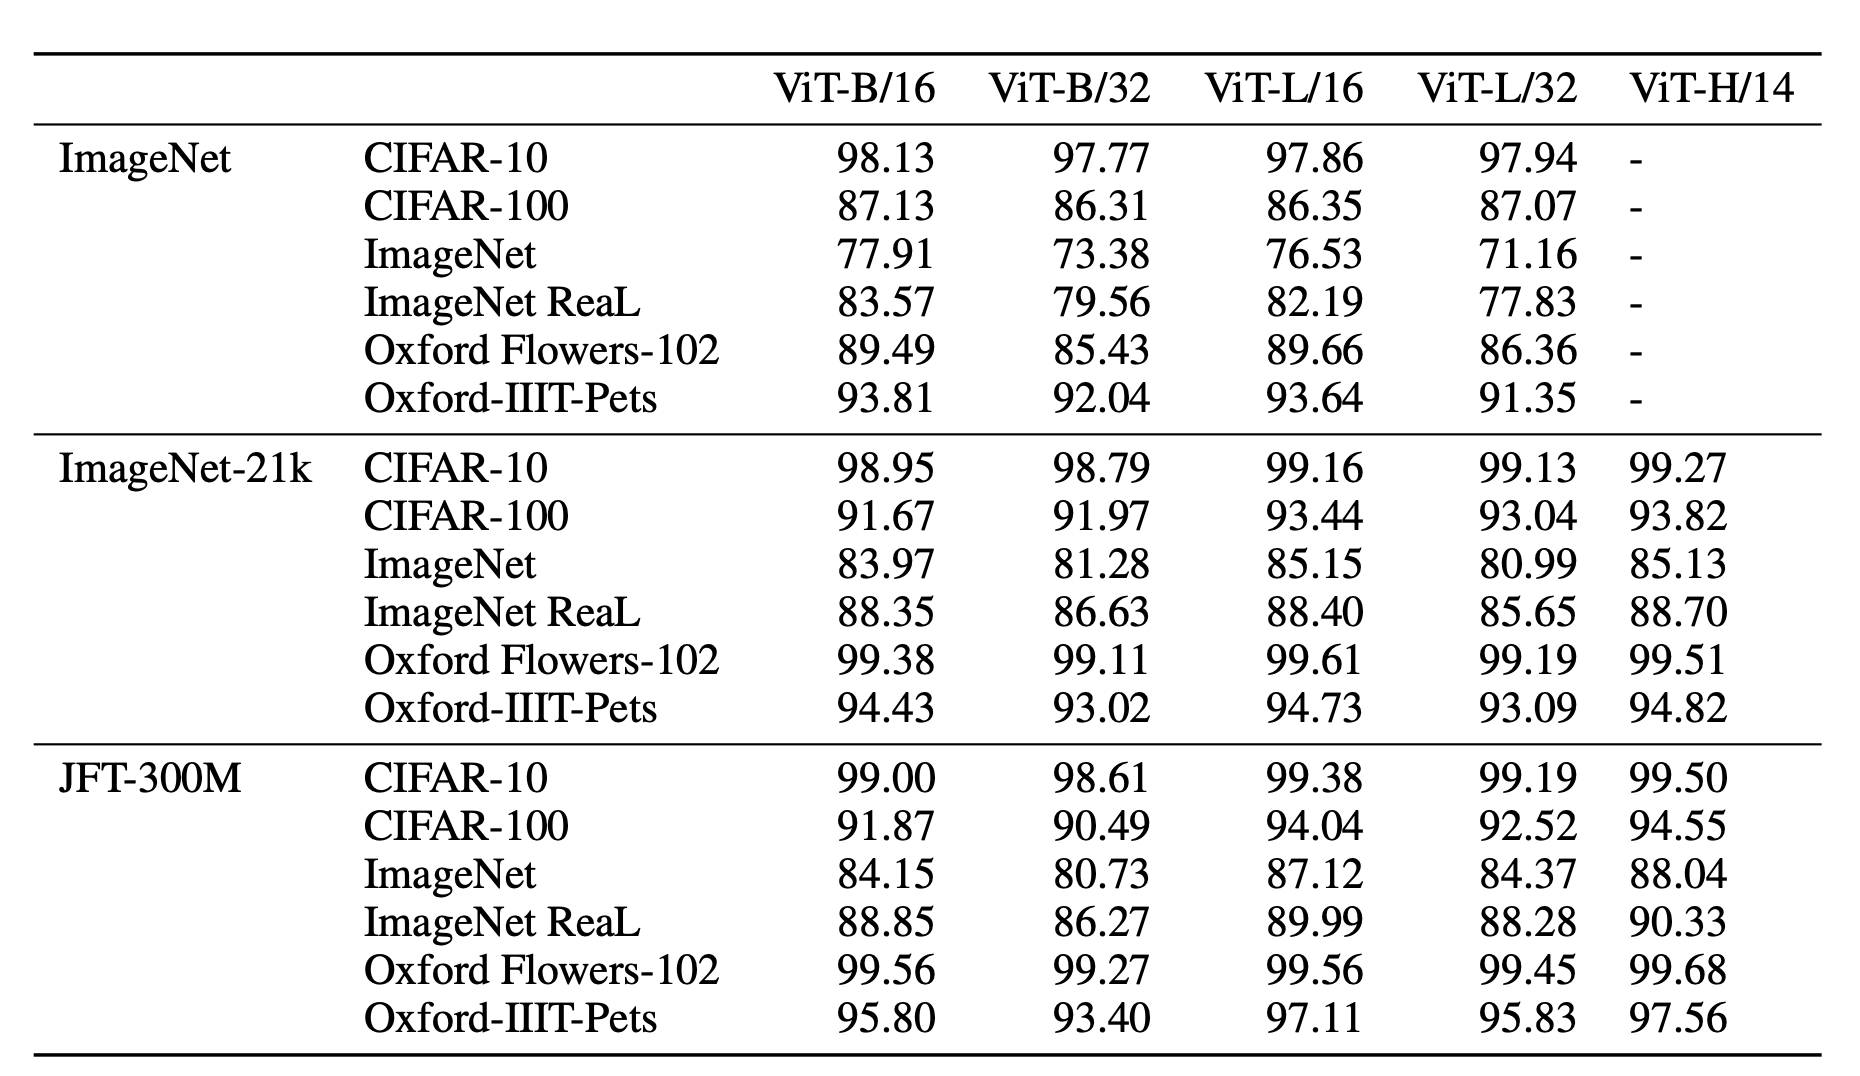
\includegraphics[width=1\textwidth]{img/4-section/More-benchmark_2.png}
\end{center}

\end{frame}


\begin{frame}
\frametitle{Current top 3 Image Classification on ImageNet 1k}
Data has been acquired by the popular "\href{https://paperswithcode.com/sota/image-classification-on-imagenet?tag_filter=171}{Papers with Code}" website.


\begin{itemize}
    \item \textbf{1st place:} \textit{PeCo} with 88.3\% top-1 accuracy (ViT-H)
    \item \textbf{2nd place:} \textit{MAE} with 87.8\% top-1 accuracy (ViT-H)
    \item \textbf{3rd place:} \textit{PeCo} with 87.5\% top-1 accuracy (ViT-H)
\end{itemize}

\end{frame}

\begin{frame}
\frametitle{Current top 3 Image Classification on ImageNet 22k}
Data has been acquired by the popular "\href{https://paperswithcode.com/sota/image-classification-on-imagenet}{Papers with Code}" website.


\begin{itemize}
    \item \textbf{1st place:} \textit{OmniVec} 92.4\% accuracy (ViT)
    \item \textbf{1st place:} \textit{BASIC-L} 91.1\% accuracy (ViT)
    \item \textbf{1st place:} \textit{CoCa} 91.0\% accuracy (Multimodal with a ViT)
\end{itemize}

Best ResNet still below 90\% accuracy, best CNN-like RevCol-H 90.0\% accuracy.

\end{frame}

\begin{frame}{Self-Attention in Vision Transformers}
    \begin{itemize}
        \item \textbf{Attention Distance:} 
        \begin{itemize}
            \item Analogous to receptive field size in CNNs.
            \item Computed based on attention weights.
        \end{itemize}
        \item \textbf{Observations:}
        \begin{itemize}
            \item Some heads attend to most of the image in the lowest layers, indicating global information integration.
            \item Other heads show small attention distances in low layers.
            \item Highly localized attention is less prominent in hybrid models with a preceding ResNet.
        \end{itemize}
        \item Localized attention in low layers may serve a similar function to early convolutional layers in CNNs.
        \item \textbf{Depth:} Attention distance increases with network \textbf{depth}.
    \end{itemize}
\end{frame}